\documentclass[a4paper,11pt]{article}

\usepackage[french]{babel}
\usepackage[T1]{fontenc}
\usepackage[utf8]{inputenc}
\usepackage{graphicx}
\usepackage{listings}
%\usepackage{fullpage}

\lstset{frame=single}

\begin{document}

\title{Projet FMIN311\\Extraction de Connaissances à partir de Données\\\textbf{Classification de documents}}
\author{Geoffrey Dumas\\Olivier Saint-Paul\\Quentin Philbert\\Thibaut Castanié}
\date{Mars 2015}

\maketitle
\thispagestyle{empty}

\newpage


\setcounter{page}{1}
\tableofcontents

\newpage

\section*{Introduction}
Le but de ce projet consiste à mettre en oeuvre et évaluer une méthode de classification de documents par thème ou opinion. Le programme  permettant la transformation des documents texte en document de format .arff que nous avons développé est en Java. Les documents sont au format texte.

Nous avons donc cherché un sujet pertinent pour cet exercice qui nous a été proposé : celui du sport. Nous avons constitué un corpus de textes contenant 62 textes : 20 concernant le basketball, 20 concernant le tennis et 22 concernant le rugby. Ce choix de sports est pertinent car chaque sport a ses particularités tout en ayant des points communs, comme un ballon pour le rugby et basketball, des points pour le tennis et le basketball, etc ...

\newpage

\section{Constitution du corpus}
Nous avons récupéré la totalité des textes de nos corpus sur le site l’Équipe.fr, en ne récupérant que les articles parlant des résultats et des résumés des rencontres. Dans chaque article, nous avons récupéré le contenu que nous avons collé dans un fichier texte. Puis nous avons supprimé les informations parasites, telles les légendes des images et les textes pour partager sur les réseaux sociaux. Nous avons ainsi récupéré ainsi 20 textes de résultats de tennis, 20 de basketball et 22 de rugby, ce qui représente 62 fichiers textes nommés tennis1, tennis2, tennis3...

--screenshots--

\newpage
\section{Transformation des données en format .arff}
\subsection{Présentation du format .arff}
Un fichier .arff (Attribute-Relation File Format) est un fichier texte qui représente une liste d’instances qui partagent un ensemble d’attributs. Il est composé de deux parties principales : une en-tête et un corps contenant les données.
L’en-tête contient le nom du fichier précédé de la mention @relation, suivi de la liste des attributs et de leur type, précédés chacun de la mention @attribute.\\

\begin{lstlisting}
@relation weather

@attribute outlook {sunny, overcast, rainy}
@attribute temperature real
@attribute humidity real
@attribute windy {TRUE, FALSE}
@attribute play {yes, no}
\end{lstlisting}
\begin{center}
\textit{Exemple d'en-tête}
\end{center}

La première ligne du corps de données commence par la mention @data. Ensuite, chaque ligne contient le contenu de chaque attribut, séparé par une virgule.\\

\begin{lstlisting}
@data
sunny,85,85,FALSE,no
sunny,80,90,TRUE,no
overcast,83,86,FALSE,yes
rainy,70,96,FALSE,yes
rainy,68,80,FALSE,yes
rainy,65,70,TRUE,no
overcast,64,65,TRUE,yes
sunny,72,95,FALSE,no
sunny,69,70,FALSE,yes
rainy,75,80,FALSE,yes
sunny,75,70,TRUE,yes
overcast,72,90,TRUE,yes
overcast,81,75,FALSE,yes
rainy,71,91,TRUE,no
\end{lstlisting}
\begin{center}
\textit{Exemple d’un corps de données}
\end{center}

\subsection{Conversion des fichiers texte en fichier .arff unique}
Afin de pouvoir travailler sur le corpus sportif que nous avons créé, il nous faut créer un programme permettant de fusionner et mettre en forme les textes pour respecter la norme d’un fichier.arff.

Pour cela nous avons codé un petit analyseur en Java qui créé l’en-tête du fichier .arff, puis qui récupère le contenu de chaque fichier texte et le met sur une ligne, suivie de sa classe.\\Le code du programme est donné en annexe.

\newpage
\section{Mise en œuvre des algorithmes de classification}
\subsection{Définitions}
\paragraph{Algorithme NaïveBayes}
La classification naïve bayésienne est un type de classification probabiliste simple basée sur le théorème de Bayes avec une forte indépendance des hypothèses.

\paragraph{Machines à support de vecteurs (SVM)}
Les SVM sont des classificateurs qui reposent sur deux idées clés :
\begin{itemize}
\item La notion de marge maximale. La marge est la distance entre la frontière de séparation et les échantillons les plus proches. Ces derniers sont appelés vecteurs supports. Dans les SVM, la frontière de séparation est choisie comme celle qui maximise la marge. Le problème est de trouver la frontière séparatrice optimale, à partir d’un ensemble d’apprentissage. Cependant il existe déjà des algorithmes pour résoudre ce problème
Transformer l’espace de représentation des données d’entrées en un espace de plus grande dimension, dans lequel il est probable qu’il existe une séparatrice linéaire.
\end{itemize}
Sous weka, l’algorithme implémentant cette méthode est nommé SMO.

\paragraph{K plus proche voisin (KNN)}
L’algorithme KNN figure parmi les plus simples algorithmes d’apprentissage artificiel. Dans un contexte de classification d’une nouvelle observation x, l’idée fondatrice simple est de faire voter les plus proches voisins de cette observation. La classe de x est déterminée en fonction de la classe majoritaire parmi les k plus proches voisins de l’observation x. La méthode KNN est donc une méthode à base de voisinage, non paramétrique.\\Dans weka, l’algorithme implémentant cette méthode est nommé IBk.

\paragraph{Arbre de décision}
Cet algorithme utilise une structure d’arbre. L’extrémité de chaque branche représente les différents résultats possibles en fonction des décisions prises à chaque étape. Cet algorithme répartit une population d’individus en groupes homogènes, selon un ensemble de variables discriminantes en fonction d’un objectif fixé et connu.\\Dans weka, l’algorithme implémentant cette méthode est nommé j48.

\newpage
\section{Mise en œuvre des algorithmes de classification}
\subsection{Textes brut}
\subsection{Textes lemmatisés}
\subsection{Textes lemmatisés avec analyse morpho-syntaxique (TreeTagger)}


\newpage
\section*{Annexes}
\subsection*{Code java permettant de convertir les fichiers textes en un fichier .arff}

\begin{lstlisting}[language=Java,frame=none]
package ArffCreatorFromTextFiles;

import java.io.BufferedReader;
import java.io.File;
import java.io.FileNotFoundException;
import java.io.FileOutputStream;
import java.io.FileReader;
import java.io.IOException;
import java.io.PrintStream;

public class Main {
  public static void charger(String path) {
    // on set le system.out en mettant le fichier arff
    // que l'on souhaite en sortie
    try {
      System.setOut(new PrintStream(
        new FileOutputStream(path+"/../fichier.arff"))
      );
    } 
    catch (FileNotFoundException e) {
      e.printStackTrace();
    }
    
    // on lui ajoute l'entete
    System.out.println("@relation sport");
    System.out.println("");
    System.out.println("@attribute document_content string");
    System.out.println(
      "@attribute document_class {basketball,tennis,rugby}"
    );
    System.out.println("");
    System.out.println("@data");
    
    File corpus = new File(path);
    String [] listeRep;
    listeRep = corpus.list();
    
    // pour chaque repertoire...
    for (int i = 0; i < listeRep.length; i++) {
      File sport = new File(path+"/"+listeRep[i]);
      String[] listeTextes = sport.list();
      String line;
      BufferedReader buff = null;
      // ... on prends chaque texte ...
      for (int j = 0; j < listeTextes.length; j++) {
        String content = "";
        String titre = listeTextes[j];
        try {
          //...on recupere la ligne du fichier texte
          //et on la "nettoie" un peu...
          buff = new BufferedReader(new FileReader(sport+"/"+titre));
          while((line = buff.readLine()) != null) {
            line += " ";
            line = line.replace("\"", "");
            content += line;
          }
        } 
        catch (FileNotFoundException e) {
          e.printStackTrace();
        } 
        catch (IOException e) {
          e.printStackTrace();
        }
        //...et on y ajoute le contenu du texte ainsi
        //que sa categorie dans le fichier arff
        System.out.println('"'+content+'"'+","+sport.getName());
      }
      
    }
  }
    
  public static void main(String[] args){
    charger("/auto_home/qphilbert/EC/corpus");
  } 
}
\end{lstlisting}

\newpage
\subsection*{Tableaux d'analyse}

%\begin{center}
%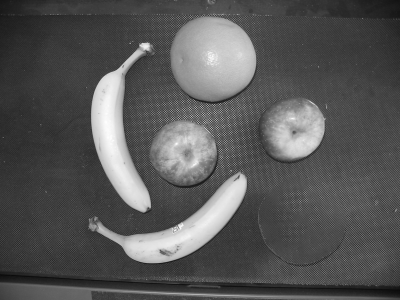
\includegraphics[scale=0.7]{fruit1_photo.png}
%\end{center}

\end{document}